\documentclass[presentation]{beamer}

\usepackage{tikz}
\usetikzlibrary{positioning,calc}
\usetikzlibrary{shapes.geometric}
\usetikzlibrary{backgrounds}% only to show the bounding box
\usetikzlibrary{shapes,arrows}
\usepackage{pgfplots}
\usepackage{pgfplotstable}
\usetikzlibrary{pgfplots.groupplots}
\pgfplotsset{compat=1.12}
\usepackage{appendixnumberbeamer}
\usepackage{amsmath}
\date{28th March 2017}
\usetheme{firedrake}

\renewcommand{\vec}[1]{\ensuremath{\boldsymbol{#1}}}
\newcommand{\ddt}[1]{\frac{\partial #1}{\partial t}}
\newcommand{\zhat}{\hat{\vec{z}}}
\newcommand{\W}{\ensuremath{\mathbb{W}}}

\newcommand{\inner}[1]{\left\langle #1 \right \rangle}

\newcommand{\KSP}[2]{\ensuremath{\mathcal{K}\left(#1, \mathbb{#2}\right)}}
\newcommand{\ksp}[1]{\KSP{#1}{#1}}

\newcommand{\highlight}[1]{\colorbox{red!20}{\color{black} #1}}

\author{Lawrence Mitchell\inst{1,*} \and Rob Kirby\inst{2}}
\institute{
\inst{1}Departments of Computing and Mathematics, Imperial College
London

\inst{*}\texttt{lawrence.mitchell@imperial.ac.uk}
\and
\inst{2}Department of Mathematics, Baylor University
}

\graphicspath{{./\jobname.figures/}}

\usepackage[url=false,
            doi=true,
            isbn=false,
            style=authoryear,
            firstinits=true,
            uniquename=init,
            backend=biber]{biblatex}

\setbeamertemplate{bibliography item}{}
\renewcommand{\bibfont}{\footnotesize}
\addbibresource{references.bib}

\setlength{\bibitemsep}{1ex}
\setlength{\fboxsep}{1pt}

\renewbibmacro{in:}{}
\DeclareFieldFormat[article]{volume}{\textbf{#1}}
\DeclareFieldFormat{doi}{%
  doi\addcolon%
  {\scriptsize\ifhyperref{\href{http://dx.doi.org/#1}{\nolinkurl{#1}}}
    {\nolinkurl{#1}}}}
\AtEveryBibitem{%
\clearfield{pages}%
\clearfield{issue}%
\clearfield{number}%
}

\usepackage{minted}

\title{Composable block preconditioning for multiphysics problems}
\subtitle{$\dots$ or, programming your solver}
\begin{document}

\maketitle

\begin{frame}[fragile]
  \frametitle{Firedrake simplifies writing models}
  \begin{columns}
    \begin{column}{0.47\framewidth}
      \begin{block}{Stationary Rayleigh-B\'enard convection}
        \begin{equation*}
          \begin{split}
            -\Delta u + u\cdot\nabla u + \nabla p +
            \frac{\text{Ra}}{\text{Pr}} \hat{g}T &= 0 \\
            \nabla \cdot u &= 0 \\
            - \frac{1}{\text{Pr}} \Delta T + u\cdot \nabla T &= 0
          \end{split}
        \end{equation*}
      \end{block}
    \end{column}
    \begin{column}{0.52\framewidth}
\begin{minted}[fontsize=\tiny,mathescape]{python}
from firedrake import *
mesh = Mesh(...)
V = VectorFunctionSpace(mesh, "CG", 2)
W = FunctionSpace(mesh, "CG", 1)
Q = FunctionSpace(mesh, "CG", 1)
Z = V * W * Q
upT = Function(Z)
u, p, T = split(upT)
v, q, S = TestFunctions(Z)
bcs = [...] # no-flow + temp gradient
nullspace = MixedVectorSpaceBasis(
   Z, [Z.sub(0), VectorSpaceBasis(constant=True), 
       Z.sub(2)])
F = (inner(grad(u), grad(v))
     + inner(dot(grad(u), u), v)
     - inner(p, div(v))
     + (Ra/Pr)*inner(T*g, v)
     + inner(div(u), q)
     + inner(dot(grad(T), u), S)
     + (1/Pr) * inner(grad(T), grad(S)))*dx

solve(F == 0, upT, bcs=bcs, nullspace=nullspace)
\end{minted}
    \end{column}
  \end{columns}
\end{frame}
\begin{frame}[standout]
  Krylov solvers are not solvers
\end{frame}

\begin{frame}
  \frametitle{It's all about preconditioning}
  \begin{itemize}
  \item Coupled problems are (typically) not amenable to black box solution
    methods.
  \item For small problems, can just use LU factorisation.
  \item For large problems, often use approximate block factorisations.
  \item Many configuration options, may require problem-specific
    auxiliary operators.
  \item Important to capture the abstraction so that automated model
    manipulation is still possible.
  \end{itemize}
\end{frame}

\begin{frame}
  \frametitle{Block preconditioning}
  Most state of the art preconditioning for multi-variable
  problems is based on block LU factorisations.

  \begin{uncoverenv}<2>
    \begin{equation*}
      T = \begin{bmatrix}
        A & 0 \\
        0 & C A^{-1} B^T
      \end{bmatrix}^{-1}
      \begin{bmatrix}
        A & B^T \\
        C & D = 0
      \end{bmatrix}
    \end{equation*}
    has minimal polynomial $T(T - I)(T^2 - T - I) =
    0$ \parencite{Murphy:2000}. \textcite{Ipsen:2001} treats case of
    $D \ne 0$.

    Alternate approach: ``function space''
    preconditioning \parencite{Kirby:2010,Mardal:2011,Malek:2014}.
  \end{uncoverenv}
\end{frame}

\begin{frame}
  \frametitle{Consequences}
  \begin{itemize}
  \item The most efficient (time to solution) strategy is problem and
    parameter dependent:
    \begin{itemize}
    \item Do I invert the blocks well or not?
    \item How many couping terms should I drop?
    \end{itemize}
  \item Need to be able to \emph{configure} the solver without
    changing the code (e.g.~eliminating first row or second?)
  \item Need to treat nested problems (Navier-Stokes inside
    Rayleigh-B\'enard).
  \item Much larger configuration space than single-variable, fully
    ``algebraic'' preconditioning.
  \end{itemize}
\end{frame}

\begin{frame}
  \frametitle{Back to Rayleigh-B\'enard}
  Newton updates need inverse of Jacobian:
  \begin{equation*}
    J = \begin{bmatrix}
      F   & B^T & M_1 \\
      C   & 0   & 0   \\
      M_2 & 0   & K
    \end{bmatrix}.
  \end{equation*}
  \begin{itemize}
  \item Navier-Stokes (top left)
  \item Convection-diffusion for temperature (bottom right)
  \item Coupling in $M_1$ and $M_2$ (non-symmetric).
  \end{itemize}
\end{frame}

\begin{frame}
  \frametitle{Preconditioning}
  We will invert $J$ with a Krylov method, so we need a
  preconditioner.
  Let
  \begin{equation*}
    N = \begin{bmatrix}
      F & B^T\\
      C & 0 \\
    \end{bmatrix} \quad
    \tilde{M}_1 =
    \begin{bmatrix}
      M_1 \\
      0
    \end{bmatrix} \quad
    \tilde{M}_2 = \begin{bmatrix}
      M_2 & 0
    \end{bmatrix}
  \end{equation*}
  and block eliminate $N$ in $J$, giving system for temperature:
  \begin{equation*}
    S_T = K - \tilde{M}_2 N^{-1} \tilde{M}_1.
  \end{equation*}
  \textcite{Howle:2012} show that $K^{-1}$ is a good preconditioner for
  $S_T$.
\end{frame}
\begin{frame}
  \frametitle{Newton update}
  Solve for the update
  \begin{equation*}
    \begin{split}
      \delta x &= J^{-1} F(x). \\
      x &\leftarrow x + \delta x
    \end{split}
  \end{equation*}

  Write $\mathcal{K}(J, \mathbb{J})$ to denote approximating $J^{-1}$
  using an iteration $\mathcal{K}$ on $J$ using $\mathbb{J}$ as a
  preconditioner.  Then the iteration
  \begin{equation*}
    \KSP{J}{\begin{bmatrix}
      \ksp{N} & 0 \\
      0 & I
    \end{bmatrix}
    \begin{bmatrix}
      I & -\tilde{M}_1 \\
      0 & I
    \end{bmatrix}
    \begin{bmatrix}
      I & 0\\
      0 & \ksp{K}
    \end{bmatrix}}
  \end{equation*}
  empirically converges swiftly, and
  requires only $\mathbb{N}$ and $\mathbb{K}$.
\end{frame}

\begin{frame}
  \frametitle{Navier-Stokes block \parencite{Elman:2014}}
  A lower Schur complement factorisation of $N$ is a good option.
  Requires $\ksp{F}$ and $\KSP{S_p}{S}$ where $S_p = -C F^{-1} B^T$.

  One option is the \emph{pressure convection-diffusion}
  approximation:
  \begin{equation*}
    \mathbb{S} = \KSP{L_p}{L} F_p \KSP{M_p}{M},
  \end{equation*}
  so our recipe for $\ksp{N}$ is:
  \begin{equation*}
    \mathcal{K}\left(N, \begin{bmatrix}
      F & 0 \\
      0 & \mathcal{K}(S_p, \KSP{L_p}{L}\,F_p \, \KSP{M_p}{M})
    \end{bmatrix}
    \begin{bmatrix}
      I & 0\\
      -C & I
    \end{bmatrix}
    \begin{bmatrix}
      \ksp{F} & 0 \\
      0 & I
    \end{bmatrix}\right).
  \end{equation*}

\end{frame}

\begin{frame}
  \frametitle{Things to note}

  \begin{itemize}
  \item We only ever need inverses of diagonal blocks.
  \item Can save memory by applying operators matrix-free.
  \item The inverses are nested, we need ways of controlling the inner
    iterations.
  \end{itemize}

  \begin{block}{PCD}
    Needs the auxiliary discretised operator $F_p$ and approximate
    inverses of the auxiliary operators $L_p$ and $M_p$.

    Communication between PDE and solver libraries can no longer be
    \emph{unidirectional}.
  \end{block}
\end{frame}

\begin{frame}
  \frametitle{Firedrake \& PETSc to the rescue}
  \begin{itemize}
  \item PETSc already provides a highly runtime-configurable library
    for \emph{algebraically} composing solvers \parencite{Brown:2012}.

  \item Firedrake makes it straightforward to build auxiliary
    operators.

  \item We combine these to allow simple development of complex
    preconditioners.
  \end{itemize}
\end{frame}
\begin{frame}
  \frametitle{Two new pieces}
 
  \begin{onlyenv}<1>
    \begin{block}{A new matrix type}
      A PETSc shell matrix that implements matrix-free actions using
      Firedrake, and contains the UFL of the bilinear form.
    \end{block}
  
  \begin{block}{Custom preconditioners}
    These matrices do not have entries, so we create custom
    preconditioners that can inspect the UFL and do the appropriate
    thing.
  \end{block}
\end{onlyenv}
\begin{onlyenv}<2>
  \begin{center}
    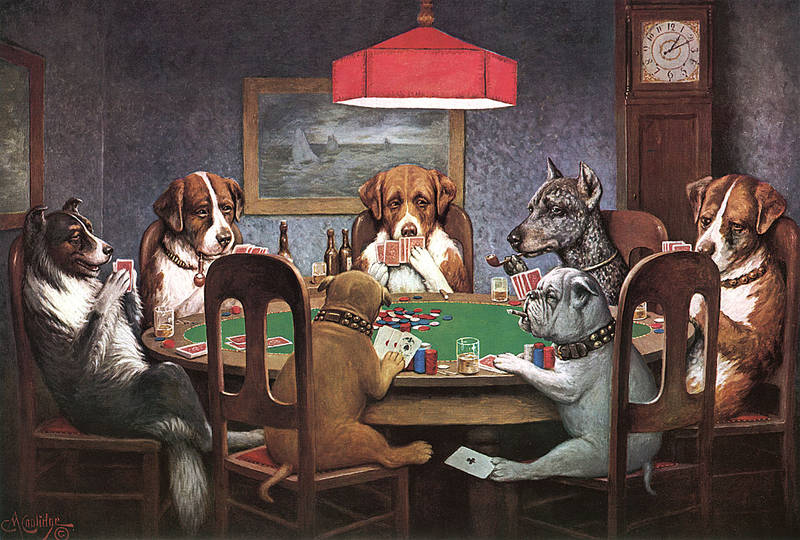
\includegraphics[width=0.8\textwidth]{underhand}
  \end{center}
\end{onlyenv}
\end{frame}


\begin{frame}[fragile]
  \frametitle{PCD}

\begin{minted}[fontsize=\tiny,mathescape]{python}
class PCDPC(PCBase):
    def initialize(self, pc):
        _, P = pc.getOperators()
        ctx = P.getContext()
        appctx = ctx.appctx
        p, q = ctx.arguments()
        [...] # Handling of boundary conditions elided
        M_p = assemble(p*q*dx)
        L_p = assemble(inner(grad(p), grad(q))*dx
        M_ksp = KSP().create()
        M_ksp.setOperators(M_p)
        L_ksp = KSP().create()
        L_ksp.setOperators(L_p)
        [...] # Some boilerplate elided
        u0 = split(appctx["state"])[appctx["velocity_space"]]
        F_p = assemble(inner(grad(p), grad(q))*dx + inner(u0, grad(p))*q*dx)

    def apply(self, pc, x, y):
        # $y \leftarrow \KSP{L_p}{L} F_p \KSP{M_p}{M} x$
        a, b = self.workspace
        self.M_ksp.solve(x, a)
        self.F_p.mult(a, b)
        self.L_ksp.solve(b, y)
\end{minted}
\end{frame}

\begin{frame}
  \frametitle{How to configure things}

  PETSc provides a ``programming language'' for configuring objects at
  runtime.  It has two operations

  \begin{enumerate}
  \item Value assignment
  \item String concatenation
  \end{enumerate}

  Every object has an \emph{options prefix} which controls where in
  the options database it looks for configuration values.

  This is verbose, but a very powerful idea.  We can control the types
  of individual solves by ensuring that they have different prefixes.
\end{frame}

\begin{frame}[fragile]
  \frametitle{The elided boilerplate}
\begin{minted}[fontsize=\small]{python}
class PCDPC(PCBase):
    def initialize(self, pc):
        ...
        prefix = pc.getOptionsPrefix()
        M_ksp.setOptionsPrefix(prefix + "pcd_Mp_")
        M_ksp.setFromOptions()
        L_ksp.setOptionsPrefix(prefix + "pcd_Lp_")
        L_ksp.setFromOptions()
\end{minted}
\end{frame}

\begin{frame}
  \frametitle{Back to the main event}
  We are solving
  \begin{equation*}
    \KSP{\begin{bmatrix}
        F & B^T & M_1\\
        C & 0 & 0 \\
        M_2 & 0 & K
      \end{bmatrix}}{J}
  \end{equation*}
  using
  \begin{equation*}
    \mathbb{J} =
    \begin{bmatrix}
      \KSP{\begin{bmatrix}
          F & B^T\\
          C & 0
        \end{bmatrix}}{N} & 0\\
      0 & I
    \end{bmatrix}
    \begin{bmatrix}
      I & 0 & -M_1\\
      0 & I & 0 \\
      0 & 0 & I
    \end{bmatrix}
    \begin{bmatrix}
      I & 0 & 0\\
      0 & I & 0\\
      0 & 0 &\ksp{K}
    \end{bmatrix}
  \end{equation*}
  with
  \begin{equation*}
    \mathbb{N} = \begin{bmatrix}
      F & 0 \\
      0 & \mathcal{K}(S_p, \KSP{L_p}{L}\,F_p \, \KSP{M_p}{M})
    \end{bmatrix}
    \begin{bmatrix}
      I & 0\\
      -C & I
    \end{bmatrix}
    \begin{bmatrix}
      \ksp{F} & 0 \\
      0 & I
    \end{bmatrix}
  \end{equation*}
  and
  \begin{equation*}
    S_p = -C \ksp{F} B^T.
  \end{equation*}
\end{frame}

\begin{frame}[fragile]
  \frametitle{First, the temperature solve}
  \small
  \begin{onlyenv}<1>
    \begin{equation*}
      \KSP{J}{%
      \begin{bmatrix}
        \KSP{\begin{bmatrix}
            F & B^T\\
            C & 0
          \end{bmatrix}}{N} & 0\\
        0 & I
      \end{bmatrix}
      \begin{bmatrix}
        I & 0 & -M_1\\
        0 & I & 0 \\
        0 & 0 & I
      \end{bmatrix}
      \begin{bmatrix}
        I & 0 & 0\\
        0 & I & 0\\
        0 & 0 &\ksp{K}
      \end{bmatrix}}
    \end{equation*}
\begin{minted}[fontsize=\tiny,escapeinside=||]{py}
-mat_type matfree
-ksp_type fgmres
-pc_type fieldsplit
-pc_fieldsplit_type multiplicative
-pc_fieldsplit_0_fields 0,1
-pc_fieldsplit_1_fields 2
-fieldsplit_1_ksp_type gmres
-fieldsplit_1_pc_type python
-fieldsplit_1_pc_python_type firedrake.AssembledPC
-fieldsplit_1_assembled_pc_type hypre
\end{minted}
  \end{onlyenv}
  \begin{onlyenv}<2>
    \color{gray}
    \begin{equation*}
      \KSP{\highlight{$J$}}{%
      \begin{bmatrix}
        \KSP{\begin{bmatrix}
            F & B^T\\
            C & 0
          \end{bmatrix}}{N} & 0\\
        0 & I
      \end{bmatrix}
      \begin{bmatrix}
        I & 0 & -M_1\\
        0 & I & 0 \\
        0 & 0 & I
      \end{bmatrix}
      \begin{bmatrix}
        I & 0 & 0\\
        0 & I & 0\\
        0 & 0 &\ksp{K}
      \end{bmatrix}}
    \end{equation*}
\begin{minted}[fontsize=\tiny,escapeinside=||]{py}
|\highlight{-mat\_type matfree}|
-ksp_type fgmres
-pc_type fieldsplit
-pc_fieldsplit_type multiplicative
-pc_fieldsplit_0_fields 0,1
-pc_fieldsplit_1_fields 2
-fieldsplit_1_ksp_type gmres
-fieldsplit_1_pc_type python
-fieldsplit_1_pc_python_type firedrake.AssembledPC
-fieldsplit_1_assembled_pc_type hypre
\end{minted}
  \end{onlyenv}
  \begin{onlyenv}<3>
    \color{gray}
    \begin{equation*}
      \highlight{$\mathcal{K}$}\left(J,%
      \begin{bmatrix}
        \KSP{\begin{bmatrix}
            F & B^T\\
            C & 0
          \end{bmatrix}}{N} & 0\\
        0 & I
      \end{bmatrix}
      \begin{bmatrix}
        I & 0 & -M_1\\
        0 & I & 0 \\
        0 & 0 & I
      \end{bmatrix}
      \begin{bmatrix}
        I & 0 & 0\\
        0 & I & 0\\
        0 & 0 &\ksp{K}
      \end{bmatrix}\right)
    \end{equation*}
\begin{minted}[fontsize=\tiny,escapeinside=||]{py}
-mat_type matfree
|\highlight{-ksp\_type fgmres}|
-pc_type fieldsplit
-pc_fieldsplit_type multiplicative
-pc_fieldsplit_0_fields 0,1
-pc_fieldsplit_1_fields 2
-fieldsplit_1_ksp_type gmres
-fieldsplit_1_pc_type python
-fieldsplit_1_pc_python_type firedrake.AssembledPC
-fieldsplit_1_assembled_pc_type hypre
\end{minted}
  \end{onlyenv}
  \begin{onlyenv}<4>
    \color{gray}
    \begin{equation*}
      \KSP{J}{%
      \highlight{$\begin{bmatrix}
        \KSP{\begin{bmatrix}
            F & B^T\\
            C & 0
          \end{bmatrix}}{N} & 0\\
        0 & I
      \end{bmatrix}
      \begin{bmatrix}
        I & 0 & -M_1\\
        0 & I & 0 \\
        0 & 0 & I
      \end{bmatrix}
      \begin{bmatrix}
        I & 0 & 0\\
        0 & I & 0\\
        0 & 0 &\ksp{K}
      \end{bmatrix}$}}
    \end{equation*}
\begin{minted}[fontsize=\tiny,escapeinside=||]{py}
-mat_type matfree
-ksp_type fgmres
|\highlight{-pc\_type fieldsplit}|
|\highlight{-pc\_fieldsplit\_type multiplicative}|
-pc_fieldsplit_0_fields 0,1
-pc_fieldsplit_1_fields 2
-fieldsplit_1_ksp_type gmres
-fieldsplit_1_pc_type python
-fieldsplit_1_pc_python_type firedrake.AssembledPC
-fieldsplit_1_assembled_pc_type hypre
\end{minted}
  \end{onlyenv}
  \begin{onlyenv}<5>
    \color{gray}
    \begin{equation*}
      \KSP{J}{%
      \begin{bmatrix}
        \highlight{$\KSP{\begin{bmatrix}
            F & B^T\\
            C & 0
          \end{bmatrix}}{N}$} & 0\\
        0 & I
      \end{bmatrix}
      \begin{bmatrix}
        I & 0 & -M_1\\
        0 & I & 0 \\
        0 & 0 & I
      \end{bmatrix}
      \begin{bmatrix}
        I & 0 & 0\\
        0 & I & 0\\
        0 & 0 &\ksp{K}
      \end{bmatrix}}
    \end{equation*}
\begin{minted}[fontsize=\tiny,escapeinside=||]{py}
-mat_type matfree
-ksp_type fgmres
-pc_type fieldsplit
-pc_fieldsplit_type multiplicative
|\highlight{-pc\_fieldsplit\_0\_fields 0,1}|
-pc_fieldsplit_1_fields 2
-fieldsplit_1_ksp_type gmres
-fieldsplit_1_pc_type python
-fieldsplit_1_pc_python_type firedrake.AssembledPC
-fieldsplit_1_assembled_pc_type hypre
\end{minted}
  \end{onlyenv}
  \begin{onlyenv}<6>
    \color{gray}
    \begin{equation*}
      \KSP{J}{%
      \begin{bmatrix}
        \KSP{\begin{bmatrix}
            F & B^T\\
            C & 0
          \end{bmatrix}}{N} & 0\\
        0 & I
      \end{bmatrix}
      \begin{bmatrix}
        I & 0 & -M_1\\
        0 & I & 0 \\
        0 & 0 & I
      \end{bmatrix}
      \begin{bmatrix}
        I & 0 & 0\\
        0 & I & 0\\
        0 & 0 & \highlight{$\ksp{K}$}
      \end{bmatrix}}
    \end{equation*}
\begin{minted}[fontsize=\tiny,escapeinside=||]{py}
-mat_type matfree
-ksp_type fgmres
-pc_type fieldsplit
-pc_fieldsplit_type multiplicative
-pc_fieldsplit_0_fields 0,1
|\highlight{-pc\_fieldsplit\_1\_fields 2}|
-fieldsplit_1_ksp_type gmres
-fieldsplit_1_pc_type python
-fieldsplit_1_pc_python_type firedrake.AssembledPC
-fieldsplit_1_assembled_pc_type hypre
\end{minted}
  \end{onlyenv}
  \begin{onlyenv}<7>
    \color{gray}
    \begin{equation*}
      \KSP{J}{%
      \begin{bmatrix}
        \KSP{\begin{bmatrix}
            F & B^T\\
            C & 0
          \end{bmatrix}}{N} & 0\\
        0 & I
      \end{bmatrix}
      \begin{bmatrix}
        I & 0 & -M_1\\
        0 & I & 0 \\
        0 & 0 & I
      \end{bmatrix}
      \begin{bmatrix}
        I & 0 & 0\\
        0 & I & 0\\
        0 & 0 & \highlight{$\mathcal{K}$}(K, \mathbb{K})
      \end{bmatrix}}
    \end{equation*}
\begin{minted}[fontsize=\tiny,escapeinside=||]{py}
-mat_type matfree
-ksp_type fgmres
-pc_type fieldsplit
-pc_fieldsplit_type multiplicative
-pc_fieldsplit_0_fields 0,1
-pc_fieldsplit_1_fields 2
|\highlight{-fieldsplit\_1\_ksp\_type gmres}|
-fieldsplit_1_pc_type python
-fieldsplit_1_pc_python_type firedrake.AssembledPC
-fieldsplit_1_assembled_pc_type hypre
\end{minted}
  \end{onlyenv}
  \begin{onlyenv}<8>
    \color{gray}
    \begin{equation*}
      \KSP{J}{%
      \begin{bmatrix}
        \KSP{\begin{bmatrix}
            F & B^T\\
            C & 0
          \end{bmatrix}}{N} & 0\\
        0 & I
      \end{bmatrix}
      \begin{bmatrix}
        I & 0 & -M_1\\
        0 & I & 0 \\
        0 & 0 & I
      \end{bmatrix}
      \begin{bmatrix}
        I & 0 & 0\\
        0 & I & 0\\
        0 & 0 & \mathcal{K}(K, \highlight{$\mathbb{K}$})
      \end{bmatrix}}
    \end{equation*}
\begin{minted}[fontsize=\tiny,escapeinside=||]{py}
-mat_type matfree
-ksp_type fgmres
-pc_type fieldsplit
-pc_fieldsplit_type multiplicative
-pc_fieldsplit_0_fields 0,1
-pc_fieldsplit_1_fields 2
-fieldsplit_1_ksp_type gmres
|\highlight{-fieldsplit\_1\_pc\_type python}|
|\highlight{-fieldsplit\_1\_pc\_python\_type firedrake.AssembledPC}|
|\highlight{-fieldsplit\_1\_assembled\_pc\_type hypre}|
\end{minted}
  \end{onlyenv}
\end{frame}

\begin{frame}[fragile]
  \frametitle{Now the Navier-Stokes block}
  \small
  \begin{onlyenv}<1>
    \begin{equation*}
      \KSP{N}{%
        \begin{bmatrix}
          F & 0 \\
          0 & \mathcal{K}(S_p, \KSP{L_p}{L}\,F_p \, \KSP{M_p}{M})
        \end{bmatrix}
        \begin{bmatrix}
          I & 0\\
          -C & I
        \end{bmatrix}
        \begin{bmatrix}
          \ksp{F} & 0 \\
          0 & I
        \end{bmatrix}}
    \end{equation*}
\begin{minted}[fontsize=\tiny,escapeinside=||]{py}
-fieldsplit_0_ksp_type gmres
-fieldsplit_0_pc_type fieldsplit
-fieldsplit_0_pc_fieldsplit_type schur
-fieldsplit_0_pc_fieldsplit_schur_fact_type lower
-fieldsplit_0_fieldsplit_0_ksp_type preonly
-fieldsplit_0_fieldsplit_0_pc_type python
-fieldsplit_0_fieldsplit_0_pc_python_type firedrake.AssembledPC
-fieldsplit_0_fieldsplit_0_assembled_pc_type hypre
-fieldsplit_0_fieldsplit_1_ksp_type preonly
-fieldsplit_0_fieldsplit_1_pc_type python
-fieldsplit_0_fieldsplit_1_pc_python_type firedrake.PCDPC
-fieldsplit_0_fieldsplit_1_pcd_Fp_mat_type matfree
-fieldsplit_0_fieldsplit_1_pcd_Mp_ksp_type preonly
-fieldsplit_0_fieldsplit_1_pcd_Mp_pc_type ilu
-fieldsplit_0_fieldsplit_1_pcd_Kp_ksp_type preonly
-fieldsplit_0_fieldsplit_1_pcd_Kp_pc_type hypre
\end{minted}
  \end{onlyenv}
  \begin{onlyenv}<2>
    \color{gray}
    \begin{equation*}
      \highlight{$\mathcal{K}$}\left(N,%
        \begin{bmatrix}
        F & 0 \\
        0 & \mathcal{K}(S_p, \KSP{L_p}{L}\,F_p \, \KSP{M_p}{M})
      \end{bmatrix}
      \begin{bmatrix}
        I & 0\\
        -C & I
      \end{bmatrix}
      \begin{bmatrix}
        \ksp{F} & 0 \\
        0 & I
      \end{bmatrix}\right)
    \end{equation*}
\begin{minted}[fontsize=\tiny,escapeinside=||]{py}
|\highlight{-fieldsplit\_0\_ksp\_type gmres}|
-fieldsplit_0_pc_type fieldsplit
-fieldsplit_0_pc_fieldsplit_type schur
-fieldsplit_0_pc_fieldsplit_schur_fact_type lower
-fieldsplit_0_fieldsplit_0_ksp_type preonly
-fieldsplit_0_fieldsplit_0_pc_type python
-fieldsplit_0_fieldsplit_0_pc_python_type firedrake.AssembledPC
-fieldsplit_0_fieldsplit_0_assembled_pc_type hypre
-fieldsplit_0_fieldsplit_1_ksp_type preonly
-fieldsplit_0_fieldsplit_1_pc_type python
-fieldsplit_0_fieldsplit_1_pc_python_type firedrake.PCDPC
-fieldsplit_0_fieldsplit_1_pcd_Fp_mat_type matfree
-fieldsplit_0_fieldsplit_1_pcd_Mp_ksp_type preonly
-fieldsplit_0_fieldsplit_1_pcd_Mp_pc_type ilu
-fieldsplit_0_fieldsplit_1_pcd_Kp_ksp_type preonly
-fieldsplit_0_fieldsplit_1_pcd_Kp_pc_type hypre
\end{minted}
  \end{onlyenv}
  \begin{onlyenv}<3>
    \color{gray}
    \begin{equation*}
      \KSP{N}{%
        \highlight{$\begin{bmatrix}
        F & 0 \\
        0 & \mathcal{K}(S_p, \KSP{L_p}{L}\,F_p \, \KSP{M_p}{M})
      \end{bmatrix}
      \begin{bmatrix}
        I & 0\\
        -C & I
      \end{bmatrix}
      \begin{bmatrix}
        \ksp{F} & 0 \\
        0 & I
      \end{bmatrix}$}}
    \end{equation*}
\begin{minted}[fontsize=\tiny,escapeinside=||]{py}
-fieldsplit_0_ksp_type gmres
|\highlight{-fieldsplit\_0\_pc\_type fieldsplit}|
|\highlight{-fieldsplit\_0\_pc\_fieldsplit\_type schur}|
|\highlight{-fieldsplit\_0\_pc\_fieldsplit\_schur\_fact\_type lower}|
-fieldsplit_0_fieldsplit_0_ksp_type preonly
-fieldsplit_0_fieldsplit_0_pc_type python
-fieldsplit_0_fieldsplit_0_pc_python_type firedrake.AssembledPC
-fieldsplit_0_fieldsplit_0_assembled_pc_type hypre
-fieldsplit_0_fieldsplit_1_ksp_type preonly
-fieldsplit_0_fieldsplit_1_pc_type python
-fieldsplit_0_fieldsplit_1_pc_python_type firedrake.PCDPC
-fieldsplit_0_fieldsplit_1_pcd_Fp_mat_type matfree
-fieldsplit_0_fieldsplit_1_pcd_Mp_ksp_type preonly
-fieldsplit_0_fieldsplit_1_pcd_Mp_pc_type ilu
-fieldsplit_0_fieldsplit_1_pcd_Kp_ksp_type preonly
-fieldsplit_0_fieldsplit_1_pcd_Kp_pc_type hypre
\end{minted}
  \end{onlyenv}
  \begin{onlyenv}<4>
    \color{gray}
    \begin{equation*}
      \KSP{N}{%
        \begin{bmatrix}
        F & 0 \\
        0 & \mathcal{K}(S_p, \KSP{L_p}{L}\,F_p \, \KSP{M_p}{M})
      \end{bmatrix}
      \begin{bmatrix}
        I & 0\\
        -C & I
      \end{bmatrix}
      \begin{bmatrix}
        \highlight{$\mathcal{K}$}(K, \mathbb{K}) & 0 \\
        0 & I
      \end{bmatrix}}
    \end{equation*}
\begin{minted}[fontsize=\tiny,escapeinside=||]{py}
-fieldsplit_0_ksp_type gmres
-fieldsplit_0_pc_type fieldsplit
-fieldsplit_0_pc_fieldsplit_type schur
-fieldsplit_0_pc_fieldsplit_schur_fact_type lower
|\highlight{-fieldsplit\_0\_fieldsplit\_0\_ksp\_type preonly}|
-fieldsplit_0_fieldsplit_0_pc_type python
-fieldsplit_0_fieldsplit_0_pc_python_type firedrake.AssembledPC
-fieldsplit_0_fieldsplit_0_assembled_pc_type hypre
-fieldsplit_0_fieldsplit_1_ksp_type preonly
-fieldsplit_0_fieldsplit_1_pc_type python
-fieldsplit_0_fieldsplit_1_pc_python_type firedrake.PCDPC
-fieldsplit_0_fieldsplit_1_pcd_Fp_mat_type matfree
-fieldsplit_0_fieldsplit_1_pcd_Mp_ksp_type preonly
-fieldsplit_0_fieldsplit_1_pcd_Mp_pc_type ilu
-fieldsplit_0_fieldsplit_1_pcd_Kp_ksp_type preonly
-fieldsplit_0_fieldsplit_1_pcd_Kp_pc_type hypre
\end{minted}
  \end{onlyenv}
  \begin{onlyenv}<5>
    \color{gray}
    \begin{equation*}
      \KSP{N}{%
        \begin{bmatrix}
        F & 0 \\
        0 & \mathcal{K}(S_p, \KSP{L_p}{L}\,F_p \, \KSP{M_p}{M})
      \end{bmatrix}
      \begin{bmatrix}
        I & 0\\
        -C & I
      \end{bmatrix}
      \begin{bmatrix}
        \mathcal{K}(F, \highlight{$\mathbb{F}$}) & 0 \\
        0 & I
      \end{bmatrix}}
    \end{equation*}
\begin{minted}[fontsize=\tiny,escapeinside=||]{py}
-fieldsplit_0_ksp_type gmres
-fieldsplit_0_pc_type fieldsplit
-fieldsplit_0_pc_fieldsplit_type schur
-fieldsplit_0_pc_fieldsplit_schur_fact_type lower
-fieldsplit_0_fieldsplit_0_ksp_type preonly
|\highlight{-fieldsplit\_0\_fieldsplit\_0\_pc\_type python}|
|\highlight{-fieldsplit\_0\_fieldsplit\_0\_pc\_python\_type firedrake.AssembledPC}|
|\highlight{-fieldsplit\_0\_fieldsplit\_0\_assembled\_pc\_type hypre}|
-fieldsplit_0_fieldsplit_1_ksp_type preonly
-fieldsplit_0_fieldsplit_1_pc_type python
-fieldsplit_0_fieldsplit_1_pc_python_type firedrake.PCDPC
-fieldsplit_0_fieldsplit_1_pcd_Fp_mat_type matfree
-fieldsplit_0_fieldsplit_1_pcd_Mp_ksp_type preonly
-fieldsplit_0_fieldsplit_1_pcd_Mp_pc_type ilu
-fieldsplit_0_fieldsplit_1_pcd_Kp_ksp_type preonly
-fieldsplit_0_fieldsplit_1_pcd_Kp_pc_type hypre
\end{minted}
  \end{onlyenv}
  \begin{onlyenv}<6>
    \color{gray}
    \begin{equation*}
      \KSP{N}{%
        \begin{bmatrix}
        F & 0 \\
        0 & \highlight{$\mathcal{K}$}(S_p, \KSP{L_p}{L}\,F_p \, \KSP{M_p}{M})
      \end{bmatrix}
      \begin{bmatrix}
        I & 0\\
        -C & I
      \end{bmatrix}
      \begin{bmatrix}
        \ksp{F} & 0 \\
        0 & I
      \end{bmatrix}}
    \end{equation*}
\begin{minted}[fontsize=\tiny,escapeinside=||]{py}
-fieldsplit_0_ksp_type gmres
-fieldsplit_0_pc_type fieldsplit
-fieldsplit_0_pc_fieldsplit_type schur
-fieldsplit_0_pc_fieldsplit_schur_fact_type lower
-fieldsplit_0_fieldsplit_0_ksp_type preonly
-fieldsplit_0_fieldsplit_0_pc_type python
-fieldsplit_0_fieldsplit_0_pc_python_type firedrake.AssembledPC
-fieldsplit_0_fieldsplit_0_assembled_pc_type hypre
|\highlight{-fieldsplit\_0\_fieldsplit\_1\_ksp\_type preonly}|
-fieldsplit_0_fieldsplit_1_pc_type python
-fieldsplit_0_fieldsplit_1_pc_python_type firedrake.PCDPC
-fieldsplit_0_fieldsplit_1_pcd_Fp_mat_type matfree
-fieldsplit_0_fieldsplit_1_pcd_Mp_ksp_type preonly
-fieldsplit_0_fieldsplit_1_pcd_Mp_pc_type ilu
-fieldsplit_0_fieldsplit_1_pcd_Kp_ksp_type preonly
-fieldsplit_0_fieldsplit_1_pcd_Kp_pc_type hypre
\end{minted}
  \end{onlyenv}
  \begin{onlyenv}<7>
    \color{gray}
    \begin{equation*}
      \KSP{N}{%
        \begin{bmatrix}
        F & 0 \\
        0 & \mathcal{K}(S_p, \highlight{$\KSP{L_p}{L}\,F_p \, \KSP{M_p}{M}$})
      \end{bmatrix}
      \begin{bmatrix}
        I & 0\\
        -C & I
      \end{bmatrix}
      \begin{bmatrix}
        \ksp{F} & 0 \\
        0 & I
      \end{bmatrix}}
    \end{equation*}
\begin{minted}[fontsize=\tiny,escapeinside=||]{py}
-fieldsplit_0_ksp_type gmres
-fieldsplit_0_pc_type fieldsplit
-fieldsplit_0_pc_fieldsplit_type schur
-fieldsplit_0_pc_fieldsplit_schur_fact_type lower
-fieldsplit_0_fieldsplit_0_ksp_type preonly
-fieldsplit_0_fieldsplit_0_pc_type python
-fieldsplit_0_fieldsplit_0_pc_python_type firedrake.AssembledPC
-fieldsplit_0_fieldsplit_0_assembled_pc_type hypre
-fieldsplit_0_fieldsplit_1_ksp_type preonly
|\highlight{-fieldsplit\_0\_fieldsplit\_1\_pc\_type python}|
|\highlight{-fieldsplit\_0\_fieldsplit\_1\_pc\_python\_type firedrake.PCDPC}|
-fieldsplit_0_fieldsplit_1_pcd_Fp_mat_type matfree
-fieldsplit_0_fieldsplit_1_pcd_Mp_ksp_type preonly
-fieldsplit_0_fieldsplit_1_pcd_Mp_pc_type ilu
-fieldsplit_0_fieldsplit_1_pcd_Kp_ksp_type preonly
-fieldsplit_0_fieldsplit_1_pcd_Kp_pc_type hypre
\end{minted}
  \end{onlyenv}
  \begin{onlyenv}<8>
    \color{gray}
    \begin{equation*}
      \KSP{N}{%
        \begin{bmatrix}
        F & 0 \\
        0 & \mathcal{K}(S_p, \KSP{L_p}{L}\,\highlight{$F_p$} \, \KSP{M_p}{M})
      \end{bmatrix}
      \begin{bmatrix}
        I & 0\\
        -C & I
      \end{bmatrix}
      \begin{bmatrix}
        \ksp{F} & 0 \\
        0 & I
      \end{bmatrix}}
    \end{equation*}
\begin{minted}[fontsize=\tiny,escapeinside=||]{py}
-fieldsplit_0_ksp_type gmres
-fieldsplit_0_pc_type fieldsplit
-fieldsplit_0_pc_fieldsplit_type schur
-fieldsplit_0_pc_fieldsplit_schur_fact_type lower
-fieldsplit_0_fieldsplit_0_ksp_type preonly
-fieldsplit_0_fieldsplit_0_pc_type python
-fieldsplit_0_fieldsplit_0_pc_python_type firedrake.AssembledPC
-fieldsplit_0_fieldsplit_0_assembled_pc_type hypre
-fieldsplit_0_fieldsplit_1_ksp_type preonly
-fieldsplit_0_fieldsplit_1_pc_type python
-fieldsplit_0_fieldsplit_1_pc_python_type firedrake.PCDPC
|\highlight{-fieldsplit\_0\_fieldsplit\_1\_pcd\_Fp\_mat\_type aij}|
-fieldsplit_0_fieldsplit_1_pcd_Mp_ksp_type preonly
-fieldsplit_0_fieldsplit_1_pcd_Mp_pc_type ilu
-fieldsplit_0_fieldsplit_1_pcd_Kp_ksp_type preonly
-fieldsplit_0_fieldsplit_1_pcd_Kp_pc_type hypre
\end{minted}
  \end{onlyenv}
  \begin{onlyenv}<9>
    \color{gray}
    \begin{equation*}
      \KSP{N}{%
      \begin{bmatrix}
        F & 0 \\
        0 & \mathcal{K}(S_p, \KSP{L_p}{L}\,F_p \, \highlight{$\mathcal{K}$}(M_p, \mathbb{M}))
      \end{bmatrix}
      \begin{bmatrix}
        I & 0\\
        -C & I
      \end{bmatrix}
      \begin{bmatrix}
        \ksp{F} & 0 \\
        0 & I
      \end{bmatrix}}
    \end{equation*}
\begin{minted}[fontsize=\tiny,escapeinside=||]{py}
-fieldsplit_0_ksp_type gmres
-fieldsplit_0_pc_type fieldsplit
-fieldsplit_0_pc_fieldsplit_type schur
-fieldsplit_0_pc_fieldsplit_schur_fact_type lower
-fieldsplit_0_fieldsplit_0_ksp_type preonly
-fieldsplit_0_fieldsplit_0_pc_type python
-fieldsplit_0_fieldsplit_0_pc_python_type firedrake.AssembledPC
-fieldsplit_0_fieldsplit_0_assembled_pc_type hypre
-fieldsplit_0_fieldsplit_1_ksp_type preonly
-fieldsplit_0_fieldsplit_1_pc_type python
-fieldsplit_0_fieldsplit_1_pc_python_type firedrake.PCDPC
-fieldsplit_0_fieldsplit_1_pcd_Fp_mat_type matfree
|\highlight{-fieldsplit\_0\_fieldsplit\_1\_pcd\_Mp\_ksp\_type preonly}|
-fieldsplit_0_fieldsplit_1_pcd_Mp_pc_type ilu
-fieldsplit_0_fieldsplit_1_pcd_Kp_ksp_type preonly
-fieldsplit_0_fieldsplit_1_pcd_Kp_pc_type hypre
\end{minted}
  \end{onlyenv}
  \begin{onlyenv}<10>
    \color{gray}
    \begin{equation*}
      \KSP{N}{%
        \begin{bmatrix}
        F & 0 \\
        0 & \mathcal{K}(S_p, \KSP{L_p}{L}\,F_p \, \mathcal{K}(M_p, \highlight{$\mathbb{M}$}))
      \end{bmatrix}
      \begin{bmatrix}
        I & 0\\
        -C & I
      \end{bmatrix}
      \begin{bmatrix}
        \ksp{F} & 0 \\
        0 & I
      \end{bmatrix}}
    \end{equation*}
\begin{minted}[fontsize=\tiny,escapeinside=||]{py}
-fieldsplit_0_ksp_type gmres
-fieldsplit_0_pc_type fieldsplit
-fieldsplit_0_pc_fieldsplit_type schur
-fieldsplit_0_pc_fieldsplit_schur_fact_type lower
-fieldsplit_0_fieldsplit_0_ksp_type preonly
-fieldsplit_0_fieldsplit_0_pc_type python
-fieldsplit_0_fieldsplit_0_pc_python_type firedrake.AssembledPC
-fieldsplit_0_fieldsplit_0_assembled_pc_type hypre
-fieldsplit_0_fieldsplit_1_ksp_type preonly
-fieldsplit_0_fieldsplit_1_pc_type python
-fieldsplit_0_fieldsplit_1_pc_python_type firedrake.PCDPC
-fieldsplit_0_fieldsplit_1_pcd_Fp_mat_type matfree
-fieldsplit_0_fieldsplit_1_pcd_Mp_ksp_type preonly
|\highlight{-fieldsplit\_0\_fieldsplit\_1\_pcd\_Mp\_pc\_type ilu}|
-fieldsplit_0_fieldsplit_1_pcd_Kp_ksp_type preonly
-fieldsplit_0_fieldsplit_1_pcd_Kp_pc_type hypre
\end{minted}
  \end{onlyenv}
  \begin{onlyenv}<11>
    \color{gray}
    \begin{equation*}
      \KSP{N}{%
        \begin{bmatrix}
        F & 0 \\
        0 & \mathcal{K}(S_p, \highlight{$\mathcal{K}$}(L_p, \mathbb{L})\,F_p \, \KSP{M_p}{M})
      \end{bmatrix}
      \begin{bmatrix}
        I & 0\\
        -C & I
      \end{bmatrix}
      \begin{bmatrix}
        \ksp{F} & 0 \\
        0 & I
      \end{bmatrix}}
    \end{equation*}
\begin{minted}[fontsize=\tiny,escapeinside=||]{py}
-fieldsplit_0_ksp_type gmres
-fieldsplit_0_pc_type fieldsplit
-fieldsplit_0_pc_fieldsplit_type schur
-fieldsplit_0_pc_fieldsplit_schur_fact_type lower
-fieldsplit_0_fieldsplit_0_ksp_type preonly
-fieldsplit_0_fieldsplit_0_pc_type python
-fieldsplit_0_fieldsplit_0_pc_python_type firedrake.AssembledPC
-fieldsplit_0_fieldsplit_0_assembled_pc_type hypre
-fieldsplit_0_fieldsplit_1_ksp_type preonly
-fieldsplit_0_fieldsplit_1_pc_type python
-fieldsplit_0_fieldsplit_1_pc_python_type firedrake.PCDPC
-fieldsplit_0_fieldsplit_1_pcd_Fp_mat_type matfree
-fieldsplit_0_fieldsplit_1_pcd_Mp_ksp_type preonly
-fieldsplit_0_fieldsplit_1_pcd_Mp_pc_type ilu
|\highlight{-fieldsplit\_0\_fieldsplit\_1\_pcd\_Kp\_ksp\_type preonly}|
-fieldsplit_0_fieldsplit_1_pcd_Kp_pc_type hypre
\end{minted}
  \end{onlyenv}
  \begin{onlyenv}<12>
    \color{gray}
    \begin{equation*}
      \KSP{N}{%
        \begin{bmatrix}
        F & 0 \\
        0 & \mathcal{K}(S_p, \mathcal{K}(L_p, \highlight{$\mathbb{L}$})\,F_p \, \KSP{M_p}{M})
      \end{bmatrix}
      \begin{bmatrix}
        I & 0\\
        -C & I
      \end{bmatrix}
      \begin{bmatrix}
        \ksp{F} & 0 \\
        0 & I
      \end{bmatrix}}
    \end{equation*}
\begin{minted}[fontsize=\tiny,escapeinside=||]{py}
-fieldsplit_0_ksp_type gmres
-fieldsplit_0_pc_type fieldsplit
-fieldsplit_0_pc_fieldsplit_type schur
-fieldsplit_0_pc_fieldsplit_schur_fact_type lower
-fieldsplit_0_fieldsplit_0_ksp_type preonly
-fieldsplit_0_fieldsplit_0_pc_type python
-fieldsplit_0_fieldsplit_0_pc_python_type firedrake.AssembledPC
-fieldsplit_0_fieldsplit_0_assembled_pc_type hypre
-fieldsplit_0_fieldsplit_1_ksp_type preonly
-fieldsplit_0_fieldsplit_1_pc_type python
-fieldsplit_0_fieldsplit_1_pc_python_type firedrake.PCDPC
-fieldsplit_0_fieldsplit_1_pcd_Fp_mat_type matfree
-fieldsplit_0_fieldsplit_1_pcd_Mp_ksp_type preonly
-fieldsplit_0_fieldsplit_1_pcd_Mp_pc_type ilu
-fieldsplit_0_fieldsplit_1_pcd_Kp_ksp_type preonly
|\highlight{-fieldsplit\_0\_fieldsplit\_1\_pcd\_Kp\_pc\_type hypre}|
\end{minted}
  \end{onlyenv}
\end{frame}

\begin{frame}
  \frametitle{Not shown}
  \begin{itemize}
  \item Setting solver tolerances
  \item Configuring $\ksp{F}$ inside application of $S_p$ (not
    needed because $\KSP{S_p}{S}$ is applied \texttt{preonly}).
  \item More complex configurations for elliptic solves
    (e.g.~$hp$-independent iterations using subspace corrections
    for high order).
  \item ...
  \end{itemize}
\end{frame}

\begin{frame}
  \frametitle{Runtime composability}

  \begin{itemize}
  \item Can tune implicit solve for Navier-Stokes on its own, then
    drop in where-ever such a block wants inverted.

  \item Model formulation doesn't care about variable
    splittings. Maybe we wanted to eliminate temperature first.  Do
    so, without changing the code.

  \item Composes with nonlinear solvers that need linearisations.

  \item Automatically take advantage of any improvements in Firedrake
    (fast matrix actions, etc...)

  \item No need to worry about parallel!
  \end{itemize}
\end{frame}

\begin{frame}
  \frametitle{Some results}
  Weak scaling for Rayleigh-B\'enard.  $\text{Ra} = 200$, $\text{Pr} =
  6.8$.  Three nonlinear iterations, 10 outer Krylov iterations.
  \begin{center}
    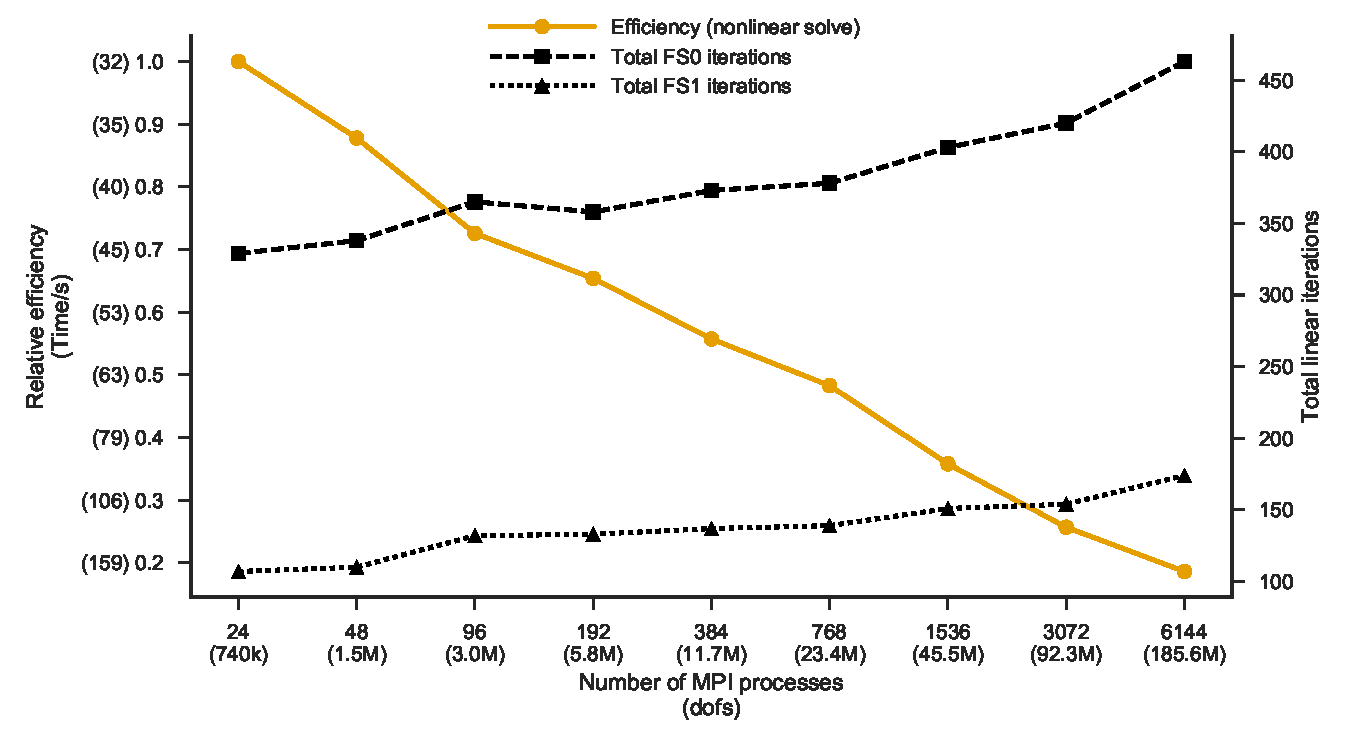
\includegraphics[width=\textwidth]{rb-weak-efficiency-Ra-200}
  \end{center}
\end{frame}

\begin{frame}[allowframebreaks]
  \frametitle{Easy extensibility}
  A preconditioner for the Ohta--Kawasaki
  equation \parencite{Farrell:2016}

  \begin{equation*}
    \begin{split}
      u_t - \Delta w + \sigma(u - m) &= 0\\
      w + \epsilon^2 \Delta u - u(u^2 - 1) &= 0
    \end{split}
  \end{equation*}
  Newton iteration at each timestep solves
  \begin{equation*}
    \begin{bmatrix}
      (1 + \Delta t \theta \sigma)M  & \Delta t\theta K \\
      -\epsilon^2 K - M_E & M
    \end{bmatrix}
    \begin{bmatrix}
      \delta u \\
      \delta w
    \end{bmatrix} =
    \begin{bmatrix}
      f_1 \\
      f_2
    \end{bmatrix}
  \end{equation*}

  \pagebreak
  
  Preconditioning
  \begin{equation*}
    P^{-1} = 
    \begin{bmatrix}
      (1 + \Delta t \theta \sigma)M  & 0 \\
      -\epsilon^2 K - M_E & S
    \end{bmatrix}^{-1} =
    \begin{bmatrix}
      A^{-1}  & 0 \\
      0 & S^{-1}
    \end{bmatrix}
    \begin{bmatrix}
      I & 0 \\
      -C A^{-1}  & I
    \end{bmatrix}.
  \end{equation*}
  Use
  \begin{equation*}
    S^{-1} \approx \hat{S}^{-1}M\hat{S}^{-1}
  \end{equation*}
  where
  \begin{equation*}
    \hat{S} = M + \epsilon\sqrt{(\Delta t \theta)/(1+\Delta t \theta\sigma)} K.
  \end{equation*}
\end{frame}

\begin{frame}[fragile]
  \frametitle{Implementation}
\begin{minted}[fontsize=\tiny,mathescape]{python}
class OKPC(PCBase):

    def initialize(self, pc):
        # Approximate $S^{-1} \sim \hat{S}^{-1} M \hat{S}^{-1}$ where $\hat{S} = \inner{q, w} + \epsilon\sqrt{c}\inner{\nabla q, \nabla w}$
        _, P = pc.getOperators()
        ctx = P.getPythonContext()
        # User information about $\Delta t$, $\theta$, etc...
        dt, theta, eps, sigma = ctx.appctx["parameters"]
        V = ctx.a.arguments()[0].function_space()
        c = (dt * theta * eps**2)/(1 + dt * theta * sigma)
        w = TrialFunction(V)
        q = TestFunction(V)
        op = assemble(inner(w, q)*dx + sqrt(c) * inner(grad(w), grad(q))*dx)
        self.ksp = KSP().create(comm=pc.comm)
        self.ksp.setOptionsPrefix(pc.getOptionsPrefix + "shat_")
        self.ksp.setOperators(op.petscmat, op.petscmat)
        [...] # boilerplate elided
        mass = assemble(w*q*dx)
        self.mass = mass.petscmat
        work = self.mass.createVecLeft()
        self.work = (work, work.duplicate())

    def apply(self, pc, x, y):
        tmp1, tmp2 = self.work
        self.ksp.solve(x, tmp1)
        self.mass.mult(tmp1, tmp2)
        self.ksp.solve(tmp2, y)
\end{minted}
\end{frame}

\begin{frame}
  \frametitle{Future directions}
  \begin{itemize}
  \item Include ability to nest multigrid solves: matrix-free multigrid.
  \item Extend approach to nonlinear preconditioning, DD (needs PyOP2++)
  \end{itemize}
  \begin{center}
    All of this is available right now

    \url{http://www.firedrakeproject.org/}
  \end{center}
\end{frame}

\begin{frame}[standout]
  Questions?
\end{frame}

\appendix
\begin{frame}[t,allowframebreaks]
  \frametitle{References}
  \printbibliography[heading=none]
\end{frame}
\end{document}
